\section{Data Pipeline}
\addcontentsline{toc}{section}{Data Pipeline}
\label{sec:data-pipeline}

\subsection{Preprocessing}
We apply several preprocessing steps to get the data into an optimal shape for our model. We also create One-hot labels.

\subsubsection{Normalization}
Normalization ensures that all images have same format.\\
One of the first steps is downsizing the images. Although our mostly high resolution pictures allow to see patterns and unique marks of the whales in great detail, we have to downsize the images enough that our memory can handle it. It is also useful to have every image in the same quadratic shape. We chose the shape (224, 224) since it is little enough to not run into memory constraints but still large enough for the model to recognize some details. The pretrained ImageNet-models also use this input size. The automatic interpolation of Tensorflow ensures that the images still look somewhat natural and not too distorted. \\
We also converted the pixel values from integers to floats to make sure that Tensorflow can work with them. The float values were fixed between -1 and 1.

\subsubsection{Foreground Extraction}
Since the images often contain much ocean in the background and the model should definitely not take this as feature, we thought it would be a good idea to crop the background such that only the whale on white background is in the image.\\
We mainly used preexisting algorithms from the Kaggle Humpback Whale challenge \cite{kapse} for this. Unfortunately, large parts of whales were cropped in many images. \\

\begin{figure}[ht] 
        \centering 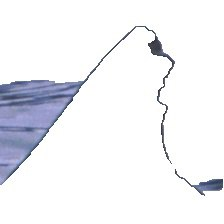
\includegraphics[width=0.7\columnwidth]{figures/whack_foreground_extraction.jpg}
        \caption{\label{fig:fe} Failed foreground extraction.}
\end{figure}

\noindent This is why we decided not to include this preprocessing step in our pipeline.

\subsubsection{Data Augmentation}
Data Augmentation has the goal of increasing the size of the data set. \\
This is especially useful for obtaining multiple images of whale individuals, for which only one or two images exist. However, we decided against data augmentation because it significantly impacted training speed - even tough we might have obtained better results with it. \\
We still decided to incorporate classic augmentation steps, such as random image flipping, contrast and brightness, to introduce more randomness to our data. This might lead to a more regularized model performance. Being nit-picky, these steps also count under "normalization", but we wanted to lay down our reasons for not doing data augmentation in a separate paragraph.

\subsection{Dataset creation}
Since online mining samples the triplets within one batch, we have to ensure on batch creation that there are sufficiently many different pairs of anchors and positives per individual within a batch. As analysed earlier, there are many individuals with only one or two images in the Happywhale data set. \\
Suddenly, this turned out to be a quite interesting constraint satisfaction problem (CSP).\\
First we had to consider what to do with the individuals with only one image, which make out 59\% of all individuals and 18\% of the dataset. One approach could be to use image augmentation and then pair the individuals with a altered version of their images. But since our model needed way to much time already, we decided to use these individuals not for training, but for another process later.

\subsubsection{Smart Batches Algorithm}
\label{subsubsec:smart-batches}
To solve this CSP, we came up with an algorithm which can easily be generalized for other triplet loss applications.

\noindent First and foremost, we decided to only accept an even batch size, which relaxes the CSP quite a lot. \\
We choose 64 as a batch size, simply because it yielded the best performance - in terms of training time - on our setup (Nvdia GTX 1080).

\noindent Let's say we have $N$ images of different animals, with at least two images per animal. We also have an even batch size $b$. We need to divide by the number of batches, which is $\lceil N/b \rceil = M$. The last batch will not have size $b$ but rather $M\%b=L$. Now we have to distribute our $N$ images over these batches in such a way, that there is never a single image of an individual in a batch and that one batch never contains images of only one individual.\\ 

\noindent The way we solve this problem is by creating \textit{two separate pools}. In the one pool we put in all the images of animals with an \textit{even} number of images and in the other all the animals with an \textit{uneven} amount of images. Then we iterate through every animal in the \textit{uneven} pool. \\
We will take the first \textit{three} images of every animal and keep them in the \textit{uneven} pool. The \textit{even} amount of rest can be thrown into the \textit{even} pool. \\
For example: If a whale has 17 images, we will keep the first $3$ pictures in the even pool and put the next $17-3=14$ pictures into the even pool. \\

\noindent Now we have only triplets left in the \textit{uneven} pool. \\
For a healthy amount of randomness, we will shuffle them around. For reproducibility, we set a seed beforehand. \\

\noindent There is a small special case when $N$ - and subsequently $L$ - is \textit{uneven}. We know that the \textit{even} pool still contains an \textit{even} amount of images. So the only source for the \textit{unevenness} of $N$ can be in the \textit{uneven} pool. This would mean that we have an \textit{uneven} amount of triplets. In this case we will just take the first triplet and put it into the last batch.\\

\noindent We have enforced that:
\begin{enumerate}
    \item Every batch has an \textit{even} amount of space left.
    \item There is an \textit{even} number of images in the \textit{even} pool
    \item There is an \textit{even} number of triplet-pairs in the (initially) \textit{uneven} pool 
\end{enumerate}

\noindent We have solved the CSP with this algorithm:

\begin{enumerate}
    \item Combine the triplet-pairs to pairs of 6 each.
    \item Distribute them over the batches.
    \item Form positive triplet-pairs of 2 in the even pool and shuffle them (with seed).
    \item We fill up the batches with the triplet-pairs of 2.
\end{enumerate}

\noindent Because we have at least two or three images of every animal in a batch, we know that that there is never a single image of an individual in a batch. Because we shuffled the first pairs of two, one batch most likely never contains images of only one individual. If this is not the case, we can simply choose another seed. To now keep this order, we will make sure to not shuffle not to shuffle at a later step in our pipeline.
